\documentclass[12pt]{article}
\usepackage{polski}
\usepackage{lmodern}
\usepackage[utf8]{inputenc}
\usepackage{tabto}
\usepackage{indentfirst} %pierwszy akapit posiada wcięcie
\usepackage{graphicx}
\title{Aproksymacja równań różniczkowych - projekt}
\author{Natalia Wojtania i Grzegorz Chojnacki}
%\date{}
\begin{document}
\maketitle

\section{Zadanie}
\subsection{Tytuł}
Tytuł zadania to ,,Metody numeryczne dla zagadnień różniczkowych".
\subsection{Treść}
Napisz program, który rozwiąże trzema metodami (Eulera, zmodyfikowaną Eulera oraz Heuna) zagadnienie różniczkowe: $$y'(x)= f(x,y(x)), y(1)=5,$$ gdzie $$ f(x,y(x))=-5x^4+2 \sqrt{y+x^5-5}+5.$$
Program ma również obliczyć dokładność dla każdej z tych metod, porównując je z dokładnym rozwiązaniem:$$ y(x)=-x^5+x^2+5.$$
\subsection{Metody}
W programie należy wykorzystać metodę Eulera, zmodyfikowaną metodę Eulera oraz metodę Heuna (udoskonaloną metodę Eulera).
\subsubsection{Opis metod}
Zagadnienie początkowe:
$$y'(x)=f(x,y(x)),y(a)=y_0$$
na przedziale $[a,b]$, gdzie $f: [a,b] \times R \rightarrow R$ jest daną funkcją, a $y_0 \in R$ jest daną liczbą.
\ Dla ustalonej liczby naturalnej $N \geq 1$ definiujemy $h= \frac{b-a}{N}$ i punkty $x_k=a+kh, 0 \leq k \leq N$ nazywane węzłami równoodległymi.
\begin{enumerate}
\item 
Metoda Eulera 
\\Jest ona metodą numeryczną do rozwiązywania równań różniczkowych z określoną wartością początkową. Metoda jest pierwszego rzędu co oznacza, że błąd lokalny (błąd na kroku) jest proporcjonalny do kwadratu wielkości kroku, a błąd globalny (błąd w danym czasie) jest proporcjonalny do wielkości kroku.
 Metoda Eulera często służy jako podstawa do konstruowania bardziej złożonych metod.

Z równania różniczkowego $y'(x)=f(x,y(x))$ dla $x=x_k$ 
\\mamy
$y'(x_k)=f(x_k,y(x_k)).$

Przybliżając $y'(x_k)$ za pomocą ilorazu różnicowego mamy
\\ $y'(x_k)\approx\frac{y(x_k+h)-y(x_k)}{h}.$

$$y(x_k+1) \approx y(x_k) +hf(x_k,y(x_k)),$$  ponieważ $x_k+h=x_{k+1}$

$$y_{k+1}=y_k +hf(x_k,y_k), 0 \leq k \leq N-1$$ 
Punkty $(x_k,y_k), 0 \leq k \leq N$ wyznaczają przybliżone rozwiązanie 
\\ $y'(x)=f(x,y(x)),y(a)=y_0$.
\item 

Zmodyfikowana metoda Eulera
\\
Metoda ta jest szczególną postacią metody Rungego-Kutty, znana popularnie jako metoda punktu środkowego.
Należy ona do klasy schematów dwustopniowych.
Wyrażona jest zależnością rekurencyją:

$$y_{k+1}=y_k +hf(x_k + \frac{h}{2},y_k + \frac{h}{2}f(x_k,y_k)), 0 \leq k \leq N-1$$ 
\item Metoda Heuna
\\W metodzie tej zamiast stałej wartości pochodnej obliczonej na początku przedziału, jak to było w metodzie   Eulera,   oblicza   się   pochodną   również   na   końcu   przedziału.   Pierwsze   oszacowanie   wyniku nazywamy predyktorem, a następnie korektorem. Metoda ta, dzięki zabiegowi numerycznemu, daje sporą zmianę w dokładności wyniku i jest znacznie dokładniejsza niż klasyczna metoda Eulera.
Wspomniany predyktor: 
$y^{Eu}_{k+1}=y_k +hf(x_k,y_k)$ wyrażamy stosując metodę Eulera.
$y'=\frac{y_k+y_{k+1}}{2}=\frac{f(x_k,y_k)+f(x_{k+1},y^{Eu}_{k+1})}{2}$ , $y^{Eu}$ liczone zwykłą metodą Eulera.\\
$y_{k+1}=y_k +\frac{h}{2}(f(x_k,y_k )+f(x_{k+1},y^{Eu}_{k+1}))$ opisuje działanie korektora.
$$y_{k+1}=y_k +\frac{h}{2}(f(x_k,y_k )+f(x_k+h,y_k+hf(x_k,y_k))), 0 \leq k \leq N-1$$  to tzw. metoda Heuna.

Te trzy metody są metodami jednokrokowymi tzn. do wyznaczenia $y_{k+1}$ potrzebny jest jeden wcześniejszy $y_k$.
\end{enumerate}


\subsubsection{Przykład}

Dla zagadnienia różniczkowego $y'(x)= f(x,y(x)), y(0)=1$
na przedziale [0,4] przyjmując krok całkowania $h = 0.5$ wyznaczyć przybliżenie $y_1$ trzema metodami oraz obliczyć błąd  $|y_1-y(x_1)|$ dla każdej z metod na tym kroku, wiedząc, że dokładne rozwiązanie to $y(x)=-\frac{1}{2}x^4+4x^3-10x^2+8.5x$ oraz  $f(x,y(x))=-2x^3+12x^2-20x+8.5 $
\\
Rozwiązanie:
\\$x_0=a=0, x_1=0+0.5=0.5, x_2=1, x_3=1.5,...,x_n=b $
\\
$y(0)=1, $
$y(x_1)=y(0.5)=-\frac{1}{2}(0.5)^4+4(0.5)^3-10(0.5)^2+8.5\cdot0.5=3.21875$
\\
\\Metoda Eulera:
$y_1=y_0+hf(x_0,y_0)$
\\
$y_1=1+0.5f(0,1)=1+0.5 \cdot 8.5 =5.25$
\\
Błąd: 
$|5.25-3.21875|=2.03125$
\\ \\Metoda punktu środkowego:
$y_1=y_0+hf(x_0+\frac{h}{2},y_0+\frac{h}{2}f(x_0,y_0))$
\\
$y_1=1+0.5f(0.25,1+0.25f(0,1))=3.109375$
\\
Błąd: 
$|3.109375-3.21875|=0.109375$
\\ \\Metoda Heuna:
$y_1=y_0 +\frac{h}{2}(f(x0,y0 )+f(x_0+h,y_0+hf(x_0,y_0)))$
\\
$y_1=1+0.25(f(0,1)+f(0.5,1+hf(0,1))=3.4375$
\\
Błąd: 
$|3.4375-3.21875|=0.21875$
\section{Opis implementacji algorytmu}
Implementacja realizująca metodę Eulera, zmodyfikowaną Eulera oraz Heuna.
\subsection{Dane wejściowe}
Na wejściu program pobiera od użytkownika liczbę $n$, określająca podział odcinka $[a, b]$ oraz liczbę $b$, informująca o końcu odcinka $[a, b]$.



\subsection{Przebieg działania}
Program wyświetla komunikat: ,,Wprowadź dane wejściowe". Jeśli zostały wprowadzone prawidłowe wartości to program poprzez funkcje \emph{euler}, \emph{eulerModified} i \emph{heun} oparte na metodzie \emph{calculate} wylicza przybliżone rozwiązania i dzięki funkcji \emph{refresh} wyświetla je wraz z błędami przybliżenia.
Próba wprowadzenia nieprawidłowych danych, które weryfikowane są w programie w funkcji \emph{refresh} skutkuje wyświetleniem stosownego ostrzeżenia.
\par Następnie funkcja \emph{calculate}  zajmuje się wyliczeniem węzłów $x_0, x_1, ... ,x_n=b$ oraz przybliżonego rozwiązania w oparciu o podaną liczbę $n$ i przedział wyznaczony przez $a=1$dane w zadaniu oraz $b$ wprowadzone przez użytkownika. 
\\
Funkcja \emph{euler} wylicza poszczególne $y_{k+1}$ metodą Eulera.
I analogicznie funkcja \emph{eulerModified} wylicza poszczególne $y_{k+1}$ zmodyfikowaną metodą Eulera. A funkcja \emph{heun} wylicza poszczególne $y_{k+1}$ metodą Eulera.



Wynikiem działania programu są przybliżone rozwiązania zagadnienia: $y'(x)= -5x^4+2 \sqrt{y+x^5-5}+5, y(1)=5$  oraz dokładność rozwiązania dla każdej z metod.
\newpage
\subsection{Najważniejsze fragmenty programu}
method.js
\begin{verbatim}

const a      = 1
const f      = (x, y) => -5*x**4 + 2*Math.sqrt(y + x**5 - 5) + 5
const yExact = x => -(x**5) + x**2 + 5
const step   = (n, b) => (b - a) / n

const calculate = (n, h, next, x = a, y = 5, error = 0) => {
  for (let k = 0; k < n; k++) {
    y = next(x, y)
    x = x + h
    error = Math.max(Math.abs(y - yExact(x)), error)
  }
  return { value: y, error: error }
}

const euler = ({n, b}) => {
  const h = step(n, b)
  const fn = (x, y) => y + h * f(x, y)
  return calculate(n, h, fn)
}

const eulerModified = ({n, b}) => {
  const h = step(n, b)
  const fn = (x, y) => y + h * f(x + h/2, y + h/2 * f(x, y))
  return calculate(n, h, fn)
}

const heun = ({n, b}) => {
  const h = step(n, b)
  const fn = (x, y) => y + h/2 * (f(x, y) + f(x + h, y + h * f(x, y)))
  return calculate(n, h, fn)
}


\end{verbatim}
\newpage
gui.js
{\footnotesize

\begin{verbatim}

const gui = new (class {
  input  = { n: document.getElementById('n'), b: document.getElementById('b') }
  output = document.getElementById('output')
  error  = document.getElementById('error')
  output = {
    euler:         document.getElementById('euler'),
    eulerModified: document.getElementById('eulerModified'),
    heun:          document.getElementById('heun')
  }

  validN = n => Number.isInteger(n) && n >= 1
  validB = b => Number.isFinite(b)  && b >= 1

  refresh() {
    const input = this.getInput()
    if (!this.validN(input.n)) this.setError('Niepaprawna wartość n')
    if (!this.validB(input.b)) this.setError('Niepaprawna wartość b')

    if (this.validB(input.b) && this.validN(input.n)) {
      this.clearError()
      this.setResult(euler(input), this.output.euler)
      this.setResult(eulerModified(input), this.output.eulerModified)
      this.setResult(heun(input), this.output.heun)
    }
  }

  setResult = (result, handle) => {
    handle.getElementsByClassName('value')[0].innerText = result.value.toFixed(2)
    handle.getElementsByClassName('error')[0].innerText = result.error.toFixed(2)
  }

  setError   = e  => this.error.innerText  = e
  clearError = () => this.error.innerText  = ''

  update = debounce(() => this.refresh(), 10)

  getInput = () => ({
     n: Number.parseFloat(this.input.n.value),
     b: Number.parseFloat(this.input.b.value)
  })
})()

\end{verbatim}
}
\newpage
\subsection{Widok działania programu}
\begin{figure}[h]
\centering
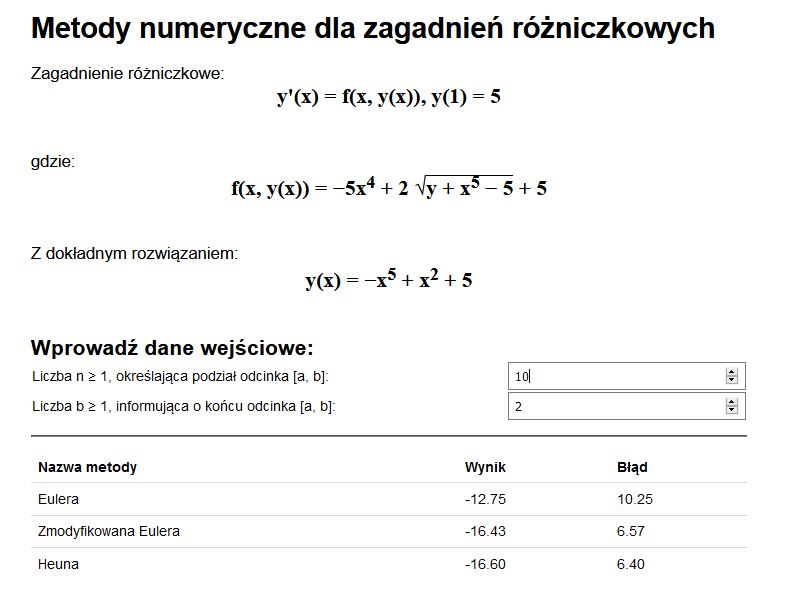
\includegraphics[scale=0.65]{correctData.jpg}
\caption{Prawidłowo wprowadzone dane}
\end{figure}

\begin{figure}
\centering
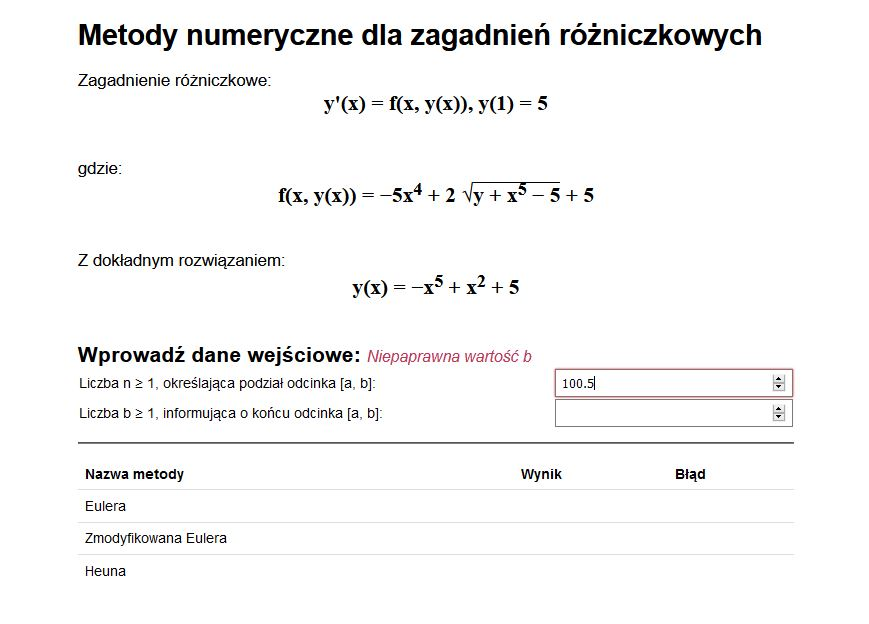
\includegraphics[scale=0.65]{wrongData.jpg}
\caption{Nieprawidłowo wprowadzona wartość n}
\end{figure}

\begin{figure}
\centering
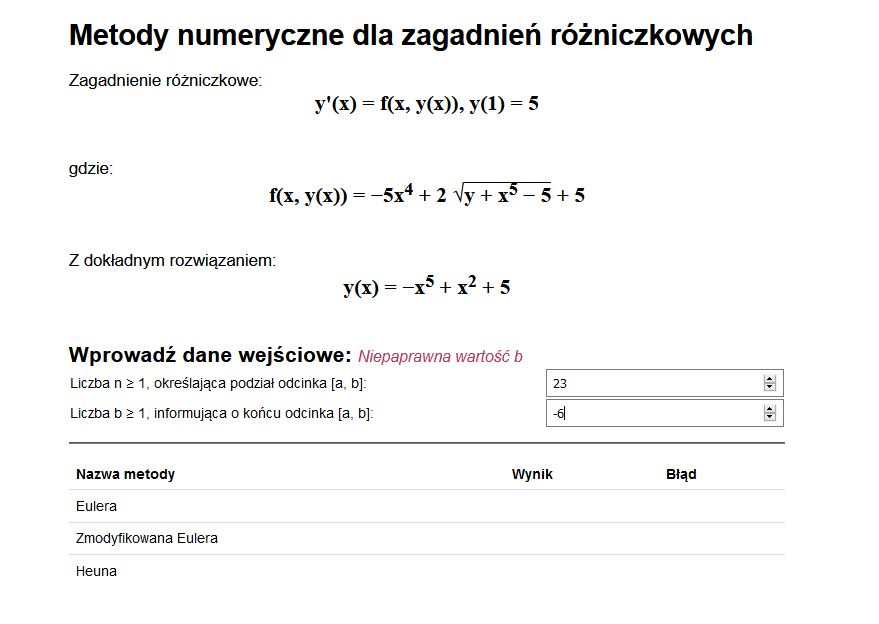
\includegraphics[scale=0.65]{wrongData2.jpg}
\caption{Nieprawidłowo wprowadzona wartość b}
\end{figure}

\end{document}
